\section{Model Driven Development (MDD)}
\subsection{Modellierung eines Embedded Systems}

\textbf{Model Driven Approach (MDA)}
\begin{itemize}
	\item Modelle werden als Werkzeuge der Dokumentation angesehen. Dadurch wird unter Umständen dasselbe zweimal beschrieben (als Code und als Diagramm)

	\item Ziel ist es aus formalen Modellen lauffähige Software zu erzeugen. Bei State Machines ist dies durch Statecharts der Automaten vollständig möglich.
\end{itemize}

\textbf{Agile Softwareentwicklung}\\
Agile Softwareentwicklung ist der Oberbegriff für den Einsatz von Agilität (flink, beweglich) in der Softwareentwicklung.
\begin{itemize}
	\item Eher offen für Änderungen als starres Festhalten an Plänen
	\item Eher Menschen und Kommunikation als Prozesse und Tools
	\item Eher "`darüber miteinander reden"' als "`gegeneinander schreiben"'
	\item Eher Vertrauen als Kontrolle
	\item Eher "`Best Practices"' aus Erfahrung als verordnete Vorgaben
	\item Eher Angemessenheit als Extremismus
	\item \textbf{Aber: keine Anarchie!}
\end{itemize}

\textbf{Model Driven Development (MDD)}\\
Bei der modellbasierten Entwicklung kommen in allen Entwicklungsphasen durchgängig Modelle zur Anwendung.

\begin{multicols}{2}
	\begin{itemize}
		\item UML:
		\begin{itemize}
			\item Aktivitätsdiagramm
			\item Sequenzdiagramm
			\item Zustandsdiagramm (Statecharts)
			\item Klassendiagramm
			\item Use Case Diagramm
			\item Verteilungsdiagramme (Deployment Diagram)
		\end{itemize}
		\item Matlab/Simulink
		\item plus evtl. weitere
	\end{itemize}
	\vfill\null
	\columnbreak

	\textbf{Generelles Vorgehen bei der Modellierung:}
	\begin{enumerate}
		\item Systemgrenze definieren (statischer Aspekt)
		\item Systemprozesse finden (statischer Aspekt)
		\item Verteilung festlegen (statischer Aspekt)
		\item Systemprozesse detaillieren (dynamischer Aspekt)
	\end{enumerate}

	\textbf{Klassifizierung von Modellierungstechniken}\\
	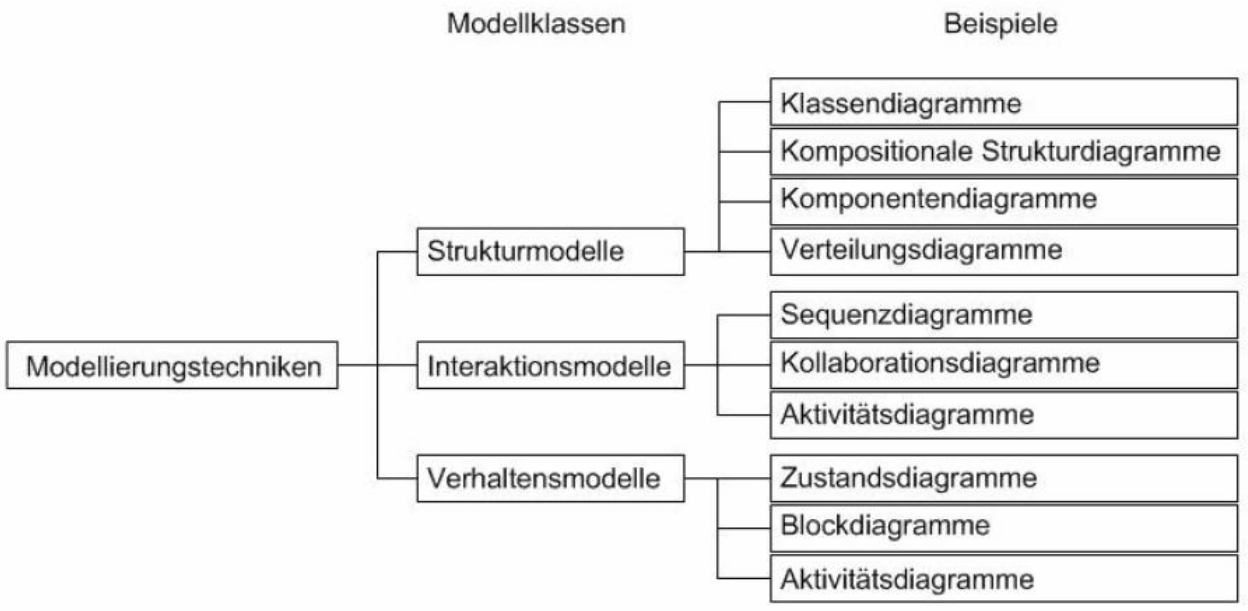
\includegraphics[width=\linewidth]{./images/Modellierung/klassifizierungModellierungstechniken}
	Wir beschäftigen uns in diesem Modul prioritär mit Interaktions- und Verhaltensmodellen, d.h. mit den dynamischen Aspekten.
\end{multicols}


\subsection{Systemgrenze definieren und Systemprozesse finden}
\subsubsection{Systemgrenze definieren}
Das wichtigste und allererste bei sämtlichen Systemen ist die Festlegung der Systemgrenze (system boundary) mittels Kontextdiagramm (\textbf{Use Case} oder auch \textbf{Sequenzdiagramm}).
\begin{itemize}
	\item Was macht das System, d.h was liegt innerhalb der Systemgrenze
	\item Mit welchen Teilen ausserhalb des Systems kommuniziert das System
	\item Welches sind die Schnittstellen zu den Nachbarsystemen
\end{itemize}

\subsubsection{Systemprozesse finden}
\begin{multicols}{2}
Die Aufteilung in Hardware und Software sollte erst nach der Analyse der grundlegenden Anforderungen erfolgen. RTE-Systeme bestehen häufig nur aus einem einzigen Systemprozess, speziell wenn das System im Prinzip 'nur' ein Regler ist. Dieser Schritt ist in der Analysephase. Wenn hier von Prozessen die Rede ist, bedeutet das nicht ein Betriebssystem-Prozess. Wichtig ist, dass es nicht zuviele Funktionsblöcke gibt (nicht ins Detail gehen). \\
Bei Systemen bei denen die Grenze durch Nachrichtenflüsse charakterisiert werden können, eignen sich \textbf{Sequenzdiagramme} zur Kontextbeschreibung.\\
\vfill\null
\columnbreak
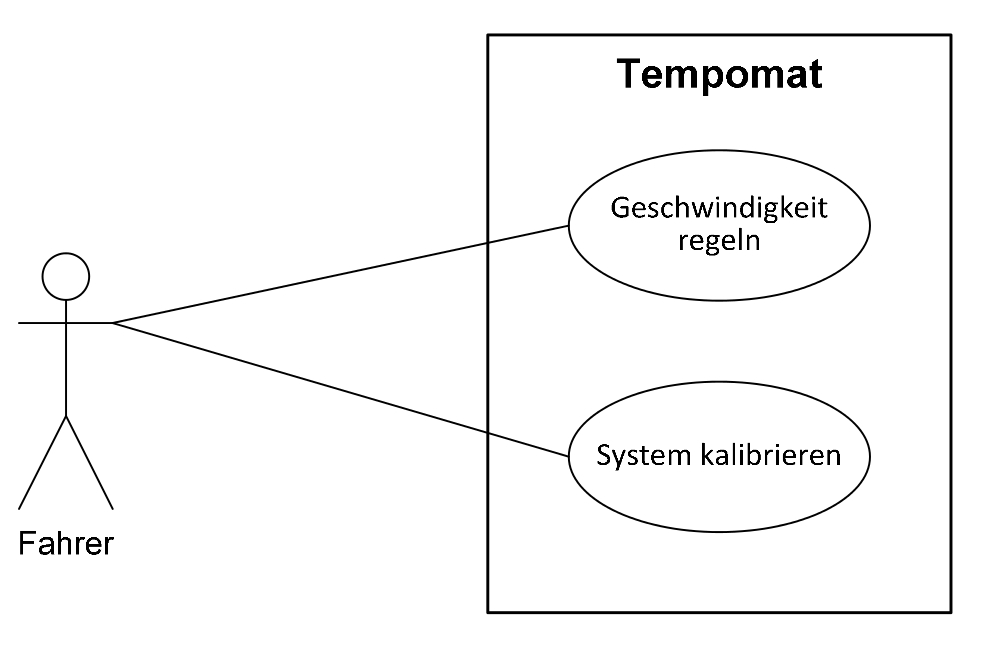
\includegraphics[height=6cm]{images/Modellierung/Systemgrenze}
\end{multicols}

\subsection{Verteilung festlegen}
Bei Embedded Systems werden häufig mehrere Rechnersysteme verwendet um die Aufgaben zu erledigen. Diese liegen meistens geografisch (cm bis km) verteilt und sind mit einem Kommunikationskanal verbunden. Diese Systeme heissen Verteilte Systeme (\textbf{Distributed Systems}). IoT-Systeme sind per Definition Verteilte Systeme.\\
Zur Darstellung eignet sich in UML das Verteilungsdiagramm (\textbf{Deployment Diagram}).

\subsubsection{Verteilungsdiagramm (Deployment Diagram)}
\begin{multicols}{2}
\begin{itemize}
	\item Die Knoten werden zur Darstellung der geografischen Orten oder Subsysteme verwendet
	\item Die physikalischen Verbindungen zwischen den Knoten (Netzwerke, Kabel, Wireless, etc.) werden als Linien dargestellt.
	\item Die Knoten können auch hierarchisch aufgebaut sein.
\end{itemize}
\vfill\null
\columnbreak
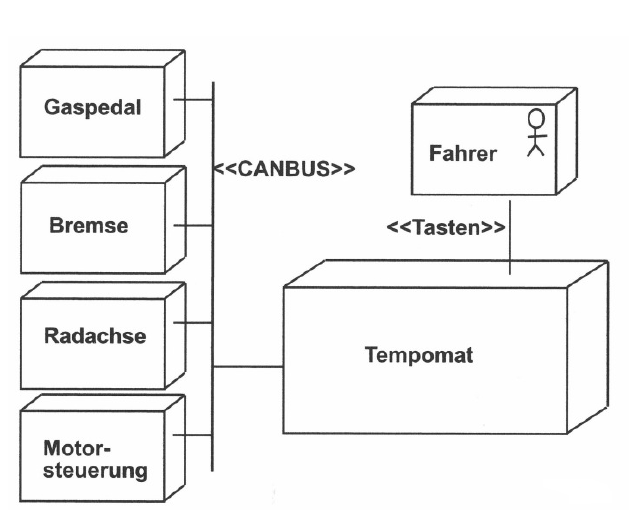
\includegraphics[height=6cm, width = 9cm,]{images/Modellierung/Verteilungsdiagramm}
\end{multicols}

\subsection{Systemprozesse Detaillieren}
Die gefundenen Systemprozesse müssen nun genauer spezifiziert werden. Dabei nicht detaillierter spezifizieren als sinnvoll. Jede weitere Detaillierung soll einen "`added value"' liefern.
Leitidee: Lieber weniger als mehr Details.

\subsubsection{Verschiedene Detaillierungsstufen}
\begin{itemize}
	\item \textbf{Überblick: } z.B in Form von normalem umgangssprachlichem Text. Diese Form sollte immer erstellt werden.
	\item \textbf{Normale Sicht: } Sie ist für den Systementwickler gedacht und enthält mehr Details.
\end{itemize}

Für die Detaillierung eignen sich umgangssprachlicher Text, Sequenzdiagramme, Aktivitätsdiagramme, Statecharts und Code (C, C++, ...).

\subsubsection{Sequenzdiagramme}

\begin{multicols}{2}
	\textbf{Zweck:}
	\begin{itemize}
		\item Austausch von Meldungen zwischen Objekten innerhalb einer beschränkten Zeitdauer anzeigen
	\end{itemize}
	\vfill\null
	\columnbreak
	\textbf{Ideal:}
	\begin{itemize}
		\item für kurze Zeitdauer mit einigen wenigen Objekten
		\item bei wenigen Verschachtelungen und Verzweigungen
	\end{itemize}
\end{multicols}

\begin{multicols}{2}
	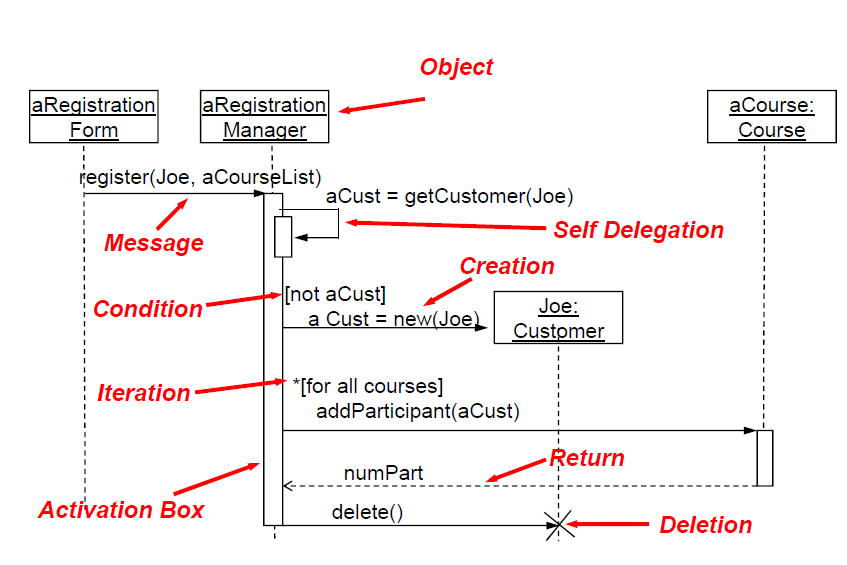
\includegraphics[width=\linewidth]{images/Modellierung/Sequenzdiagramm}
	\label{Bild1}
	\vfill\null
	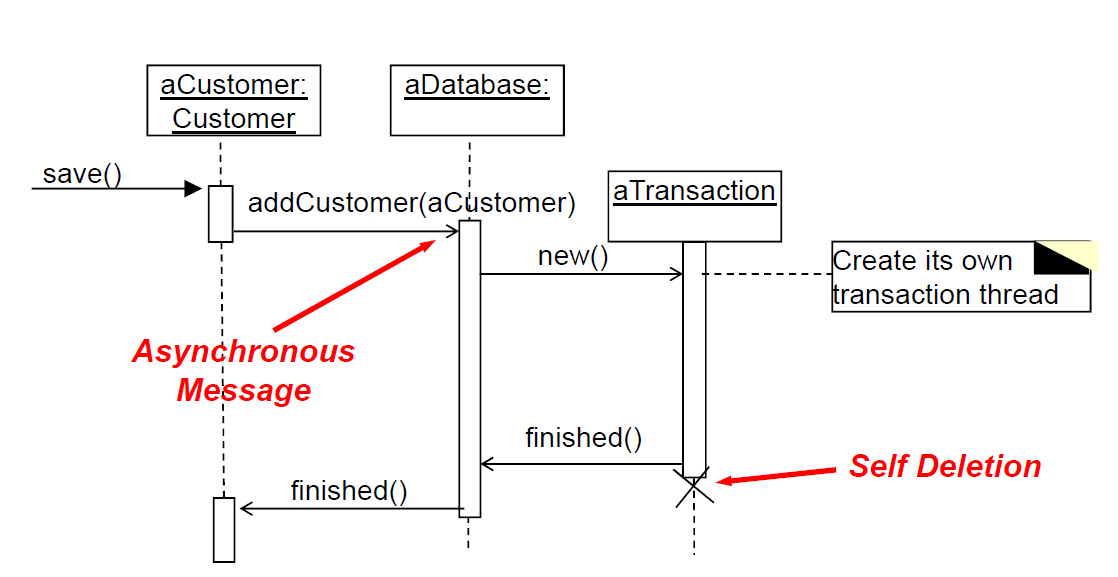
\includegraphics[width=\linewidth]{images/Modellierung/Sequenzdiagramm2}
	\label{Bild2}
\end{multicols}

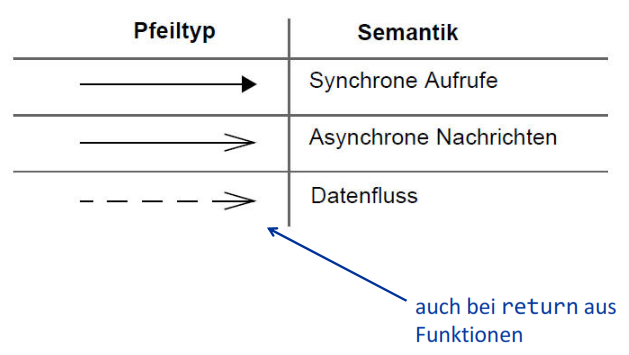
\includegraphics[width = 0.4\linewidth]{images/Modellierung/Pfeiltypen_Aktivitaetsdiagramm}

\begin{multicols}{2}
\textbf{Diagramm nicht überladen!}
\vfill\null
\columnbreak
Wann einsetzen?
\begin{itemize}
	\item Use Case Analyse (Beschreibung von Szenario)
	\item Modellierung von Nachrichtenfluss
	\item SW-Design
	\item Implementation
\end{itemize}
\end{multicols}

\newpage
\subsubsection{Kommunikationsdiagramm}
\begin{minipage}[][][t]{0.4\linewidth}
Das Kommunikationsdiagramm zeigt dieselbe Information wie das Sequenzdiagramm. Der Schwerpunkt liegt aber
nicht auf dem zeitlichen Ablauf, sondern auf dem Informationsfluss zwischen den Objekten.
\end{minipage}%
\begin{minipage}{0.6\linewidth}
\begin{center}
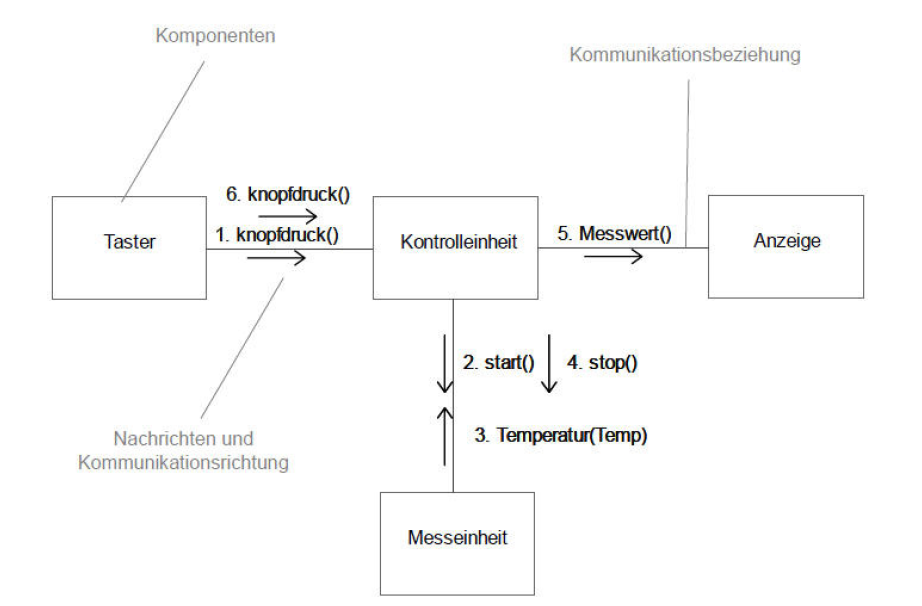
\includegraphics[width=0.8\linewidth]{images/Modellierung/Kommunikationsdiagramm}
\end{center}
\end{minipage}

\subsubsection{Aktivitätsdiagramme}
\textbf{Wird gebraucht für:}
\begin{itemize}
	\item sequenzielle Abläufe
	\item Prozess- und Steuerfluss
	\item Auch für gleichzeitige Prozesse geeignet
	\item Weniger geeignet für komplexe logische Bedingungen (Wahrheitstabelle)
\end{itemize}

\begin{multicols}{2}
	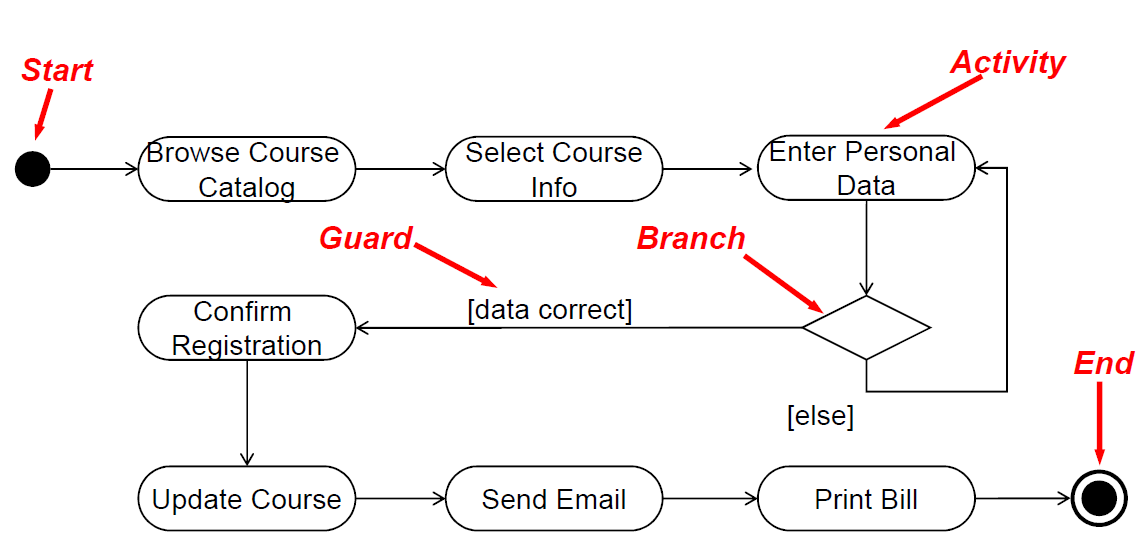
\includegraphics[width=\linewidth]{images/Modellierung/Aktivitaetsdiagramm1}
	\label{Bild3}
	\vfill\null
	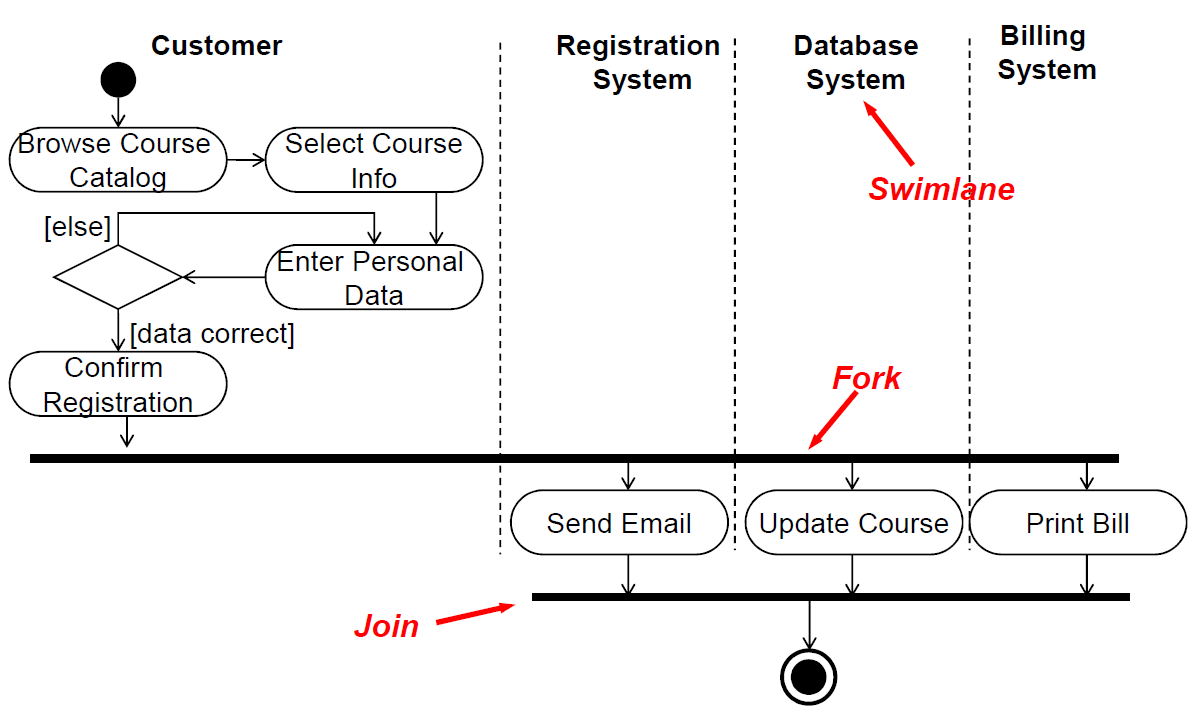
\includegraphics[width=\linewidth]{images/Modellierung/Aktivitaetsdiagramm2}
	\label{Bild4}
\end{multicols}
